% =====================================================================
% fig1_concept.tex -- Figure 1 of v14 (TikZ standalone)
%   (a) the gatekeeper: two rulebooks that accept receipts (certificates)
%   (b) "solve this puzzle, then open the safe" (program p_{e,w})
%   (c) the Goldbach plan and its bounded tests (Simulation 3)
% Compile:  pdflatex fig1_concept.tex
% The block between the AUTO-GENERATED markers in panel (c) is written by
% build_fig1_data.py from data/sim3_open_problem_results.csv.
% Do not edit that block by hand; re-run the script instead.
% =====================================================================
\documentclass[tikz,border=4pt]{standalone}
\usepackage[T1]{fontenc}
\usepackage{amsmath,amssymb}
\usetikzlibrary{arrows.meta,positioning,shapes.geometric,shapes.symbols,fit,calc}
\definecolor{allowblue}{RGB}{0,88,138}
\definecolor{denyred}{RGB}{163,41,47}
\definecolor{certorange}{RGB}{166,95,0}
\newcommand{\bad}{\mathsf{BAD}}
% one bounded test of the Goldbach plan: #1 = k, horizon H = 10^k; #2 = verdict
\newcommand{\GoldbachTest}[2]{%
  \pgfmathsetmacro{\gx}{\tlxzero+(#1-1)*\tldx}%
  \draw[thick,gray!60!black] (\gx,\tly-0.09) -- (\gx,\tly+0.09);%
  \node[lbl,anchor=north] at (\gx,\tly-0.12) {$10^{#1}$};%
  \node[verdict #2] (vt#1) at (\gx,\tly+0.62) {#2};%
  \draw[gray!60,thin] (vt#1.south) -- (\gx,\tly+0.09);%
}
\begin{document}
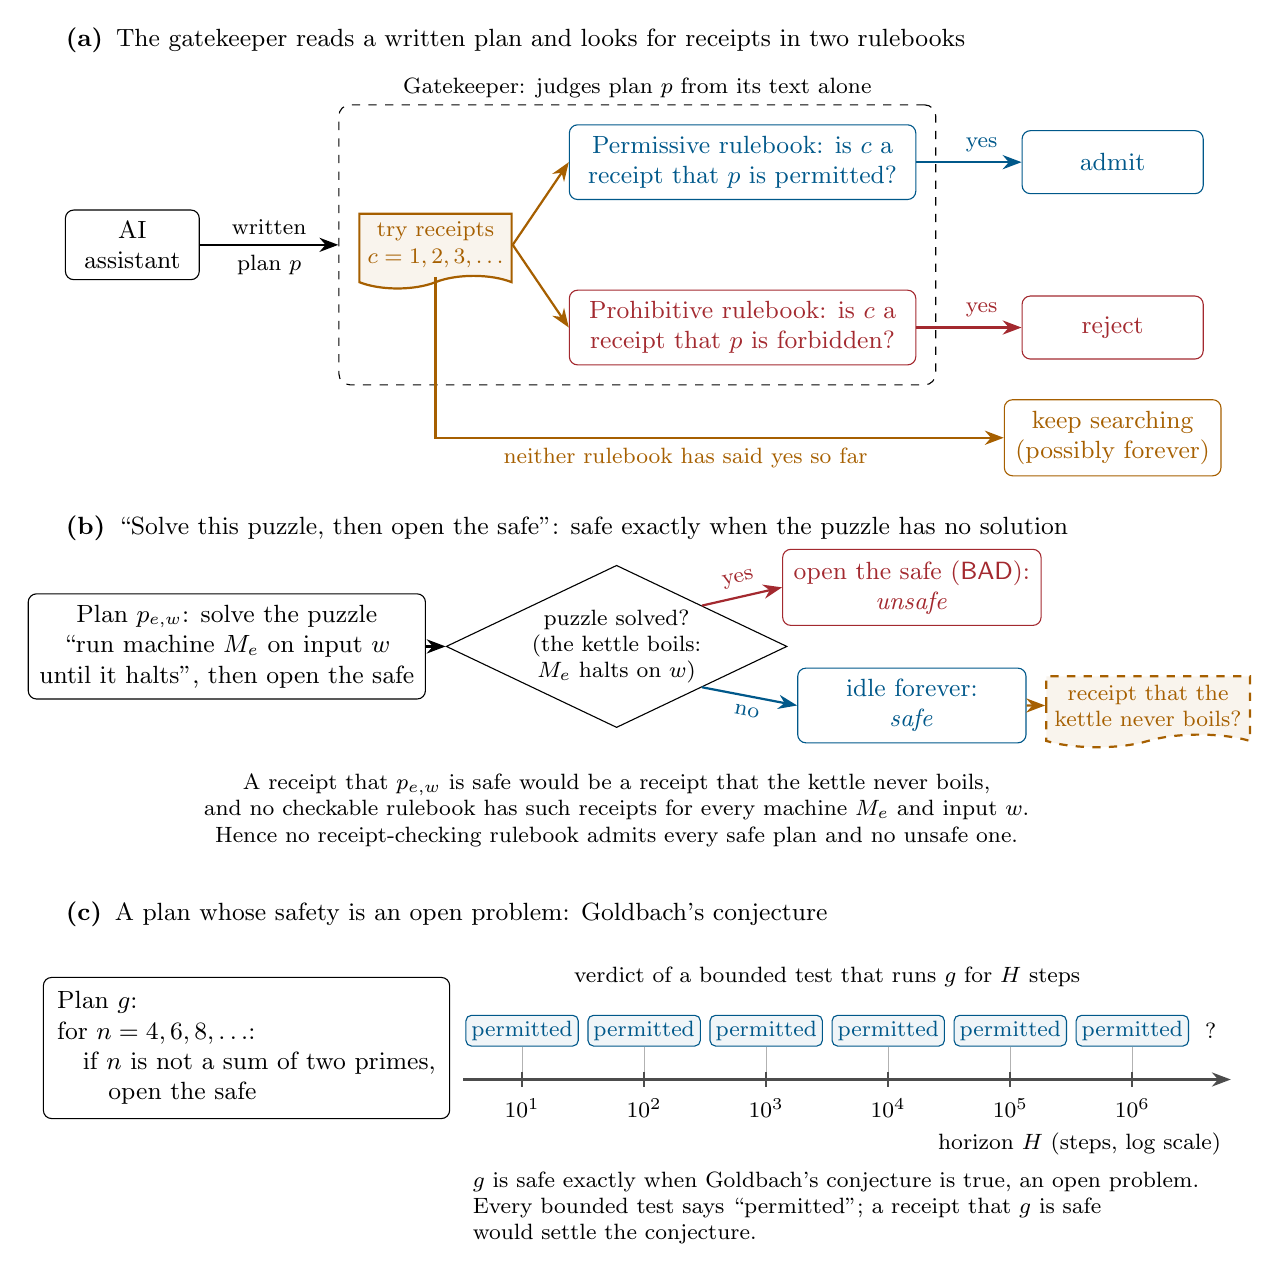
\begin{tikzpicture}[font=\small,
  box/.style={draw,rounded corners=3pt,align=center,inner sep=4pt,minimum height=8mm},
  permit/.style={box,draw=allowblue,text=allowblue},
  forbid/.style={box,draw=denyred,text=denyred},
  receipt/.style={tape,tape bend top=none,tape bend bottom=in and out,tape bend height=1.6mm,
    draw=certorange,text=certorange,fill=certorange!7,thick,align=center,inner sep=3pt,
    font=\footnotesize},
  arr/.style={-{Stealth[length=2.4mm]},thick},
  lbl/.style={font=\footnotesize,align=center},
  ptitle/.style={anchor=west,font=\small,inner sep=0pt},
  verdict permitted/.style={draw=allowblue,text=allowblue,fill=allowblue!6,rounded corners=2pt,
    font=\footnotesize,inner sep=2pt},
  verdict forbidden/.style={draw=denyred,text=denyred,fill=denyred!6,rounded corners=2pt,
    font=\footnotesize,inner sep=2pt}]

% ================================================================ Panel (a)
\node[ptitle] at (0,4.15) {\textbf{(a)}\enspace The gatekeeper reads a written plan and looks for receipts in two rulebooks};
\node[box,minimum width=17mm] (agent) at (0.85,1.55) {AI\\ assistant};
\node[receipt] (search) at (4.7,1.55) {try receipts\\ $c=1,2,3,\ldots$};
\node[permit,minimum width=44mm] (perm) at (8.6,2.6)
  {Permissive rulebook: is $c$ a\\ receipt that $p$ is permitted?};
\node[forbid,minimum width=44mm] (forb) at (8.6,0.5)
  {Prohibitive rulebook: is $c$ a\\ receipt that $p$ is forbidden?};
\node[draw,dashed,rounded corners=4pt,inner sep=7pt,fit=(search)(perm)(forb),
  label={[font=\footnotesize,anchor=south,inner sep=2pt]north:Gatekeeper: judges plan $p$ from its text alone}] (gate) {};
\draw[arr] (agent) -- node[lbl,above]{written} node[lbl,below]{plan $p$} (gate.west |- agent);
\draw[arr,certorange] (search.east) -- (perm.west);
\draw[arr,certorange] (search.east) -- (forb.west);
\node[permit,minimum width=23mm] (admit) at (13.3,2.6) {admit};
\node[forbid,minimum width=23mm] (reject) at (13.3,0.5) {reject};
\node[box,draw=certorange,text=certorange,minimum width=23mm] (wait) at (13.3,-0.9)
  {keep searching\\ (possibly forever)};
\draw[arr,allowblue] (perm) -- node[lbl,above,pos=0.62]{yes} (admit);
\draw[arr,denyred] (forb) -- node[lbl,above,pos=0.62]{yes} (reject);
\draw[arr,certorange] (search.south) |- node[lbl,pos=0.72,below]{neither rulebook has said yes so far} (wait.west);

% ================================================================ Panel (b)
\node[ptitle] at (0,-2.05) {\textbf{(b)}\enspace ``Solve this puzzle, then open the safe'': safe exactly when the puzzle has no solution};
\node[box,minimum width=40mm] (sim) at (2.05,-3.55)
  {Plan $p_{e,w}$: solve the puzzle\\ ``run machine $M_e$ on input $w$\\ until it halts'', then open the safe};
\node[draw,diamond,aspect=2.1,inner sep=1pt,align=center,font=\footnotesize] (halt) at (7.0,-3.55)
  {puzzle solved?\\ (the kettle boils:\\ $M_e$ halts on $w$)};
\node[forbid,minimum width=29mm] (bad) at (10.75,-2.8) {open the safe ($\bad$):\\ \emph{unsafe}};
\node[permit,minimum width=29mm] (safe) at (10.75,-4.3) {idle forever:\\ \emph{safe}};
\draw[arr] (sim) -- (halt);
\draw[arr,denyred] (halt.north east) -- node[lbl,above,sloped]{yes} (bad.west);
\draw[arr,allowblue] (halt.south east) -- node[lbl,below,sloped]{no} (safe.west);
\node[receipt,dashed] (nr) at (13.75,-4.3) {receipt that the\\ kettle never boils?};
\draw[arr,certorange,dashed] (safe) -- (nr);
\node[lbl,anchor=north] at (7.0,-5.05)
  {A receipt that $p_{e,w}$ is safe would be a receipt that the kettle never boils,\\
   and no checkable rulebook has such receipts for every machine $M_e$ and input $w$.\\
   Hence no receipt-checking rulebook admits every safe plan and no unsafe one.};

% ================================================================ Panel (c)
\node[ptitle] at (0,-6.95) {\textbf{(c)}\enspace A plan whose safety is an open problem: Goldbach's conjecture};
\node[box,align=left,minimum width=44mm,inner sep=5pt] (gplan) at (2.3,-8.65)
  {Plan $g$:\\ for $n = 4, 6, 8, \ldots$:\\ \quad if $n$ is not a sum of two primes,\\ \quad\quad open the safe};
\def\tly{-9.05}
\def\tlxzero{5.8}
\def\tldx{1.55}
% >>> BEGIN AUTO-GENERATED: Goldbach bounded tests
% written by build_fig1_data.py from sim3_open_problem_results.csv (program = goldbach_search); do not edit by hand
\def\GoldbachKmax{6}% largest tested exponent k (H = 10^k)
\GoldbachTest{1}{permitted}% H = 10, bad_observed = False
\GoldbachTest{2}{permitted}% H = 100, bad_observed = False
\GoldbachTest{3}{permitted}% H = 1000, bad_observed = False
\GoldbachTest{4}{permitted}% H = 10000, bad_observed = False
\GoldbachTest{5}{permitted}% H = 100000, bad_observed = False
\GoldbachTest{6}{permitted}% H = 1000000, bad_observed = False
% <<< END AUTO-GENERATED: Goldbach bounded tests
\pgfmathsetmacro{\tllast}{\tlxzero+(\GoldbachKmax-1)*\tldx}
\pgfmathsetmacro{\tlmid}{(\tlxzero+\tllast)/2}
\draw[-{Stealth[length=2.4mm]},thick,gray!60!black] (5.05,\tly) -- (\tllast+1.25,\tly);
\node[lbl,anchor=west] at (\tllast+0.8,\tly+0.62) {?};
\node[lbl,anchor=south] at (\tlmid,\tly+1.05) {verdict of a bounded test that runs $g$ for $H$ steps};
\node[lbl,anchor=north east] at (\tllast+1.25,\tly-0.55) {horizon $H$ (steps, log scale)};
\node[lbl,anchor=north west,align=left] at (5.05,\tly-1.05)
  {$g$ is safe exactly when Goldbach's conjecture is true, an open problem.\\
   Every bounded test says ``permitted''; a receipt that $g$ is safe\\ would settle the conjecture.};
\end{tikzpicture}
\end{document}
